%----------------------------------------------------------------------------------------
%	PACKAGES AND THEMES
%----------------------------------------------------------------------------------------
\documentclass[aspectratio=169,xcolor=dvipsnames]{beamer}
\usetheme{Simple}

\usepackage{hyperref}
\usepackage{graphicx} % Allows including images
\usepackage{booktabs} % Allows the use of \toprule, \midrule and \bottomrule in tables

\usepackage{graphicx}
\usepackage{subcaption}
\usepackage{mwe}

%----------------------------------------------------------------------------------------
%	TITLE PAGE
%----------------------------------------------------------------------------------------

% The title
\title[]{Auto Insurance Fraud Claim Detection}
\subtitle{}

\author[Hung Tran] {Hung Cong Tran}
%\institute[NTU] % Your institution may be shorthand to save space
%{
    % Your institution for the title page
%    Department of Computer Science and Information Engineering \\
%    National Taiwan University 
%    \vskip 3pt
%}
\date{\today} % Date, can be changed to a custom date


%----------------------------------------------------------------------------------------
%	PRESENTATION SLIDES
%----------------------------------------------------------------------------------------

\begin{document}

\begin{frame}
    % Print the title page as the first slide
    \titlepage
\end{frame}

\begin{frame}{Overview}
    % Throughout your presentation, if you choose to use \section{} and \subsection{} commands, these will automatically be printed on this slide as an overview of your presentation
    \tableofcontents
\end{frame}

%------------------------------------------------
\section{Motivation and Problem identification}
%------------------------------------------------

\begin{frame}{Motivation and Problem identification}

%\begin{enumerate*} 
Fraudulent auto insurance accident claims are very popular in India nowaday. 
\vspace{0.2in}

Insurance companies are  paying very large amounts of of wrong insurance payout and this hurts their profits significantly. 

\vspace{0.2in}

Also, insurance companies have to raise their insurance premiums and this also hurts their current customers.  

\vspace{0.2in}
Therefore, there is a big demand for a good prediction model to detect fraudulent vehicle accident claims from insurance companies.
%\end{enumerate*}

\end{frame}

\begin{frame}{Motivation and Problem identification}

In this project, I will create a classification model that help predict whether or not vehicle insurance accident claims in India are fraudulent and reduce the amount of wrong insurance payout for insurance companies.
    
\end{frame}

\section{Data}

\begin{frame}{Data}
The built model is 28836 auto insurance claims with features in four main categories as follow: 

\text{ }

\textbf{Insurance Claim Information} (e.g. Type Of Incident, Type Of Collission, Severity Of Incident, Authorities Contacted, etc) 

\text{ }

\textbf{Customer Demographics} (e.g. Insured Age, Insured ZipCode, Insured Gender, Insured Education Level, etc)

\text{ }

\textbf{Insurance Policy} (e.g. Insurance Policy Number, Customer Loyalty Period, Date Of Policy Coverage, Insurance Policy State, etc)

\text{ }

\textbf{Vehicle Information} (e.g. Vehicle Make, Vehicle Model, Vehicle Year of Model, , etc)


  
   
\end{frame}

\section{Modeling results and analysis}

\begin{frame}{Modeling results and analysis (Model selection)}
I try different classification models on the training data set and use cross-validation to compute the average AUC score. Here is the result: 

\begin{center}
\begin{tabular}{||c c||} 
 \hline
 Models & AUC scores\\ [0.5ex] 
 \hline\hline
 KNeighborsClassifier & 0.90 \\ 
 \hline
 Logistic regression & 0.79 \\
 \hline
 SVM (with polynomial kernel) & 0.91 \\
 \hline
 SVM (with radial basis function kernel) & 0.91 \\
 \hline
 Decision Tree & 0.79\\
 \hline
 Random Forrest & 0.91 \\ 
 %[1ex] 
 \hline
 AdaBoost with random forests & 0.91\\
 \hline
 GradientBoostingClassifier & 0.88\\
 \hline
 XGBoost & 0.91\\
 \hline
\end{tabular}
\end{center}

\end{frame}

\begin{frame}{Modeling results and analysis (Model selection)}
It seems that SVM, Random forest, Adaboost with random forests, and XGBoost models all perform well. For the simplicity and interpretability I choose the Random forest model to proceed.

\text{ }

After running the Grid Search to find the best random forest model, I chose the one with on 560 estimators.
\end{frame}

\begin{frame}{Modeling results and analysis (Model selection)}
The chosen model achieves the 0.92 AUC scores. We also achieved the accuracy 92\% and the precision, recall, and F1-scores as follows:

\text{ }

\text{ }

\begin{center}
\begin{tabular}{ |p{2cm}||p{2cm}|p{2cm}|p{2cm}|p{2cm}|  }
 \hline
 \multicolumn{5}{|c|}{Report for the performance on the test set} \\
 \hline
\text{ }& Precision & Recall & F1-score & Support\\
 \hline
 Not Fraud   & 0.92    &0.98&   0.95 & 3953\\
 Fraud  &   0.94  & 0.77   &0.85& 1477\\
 \hline
\end{tabular}
\end{center}

\end{frame}

\begin{frame}{Modeling results and analysis (Feature importance)}

The five most important features that came up in the modeling as follows:


\vspace{0.2in}
\begin{center}
\begin{tabular}{ |p{3cm}|p{8cm}|p{2.5cm}|  }
 \hline
 \multicolumn{3}{|c|}{Feature Importance} \\
 \hline
Rank& Feature & Contribution\\
 \hline
1 & Severity Of Incident   &       0.091433\\
2 & Insured Hobbies chess  &      0.041979\\
3 & Amount Of Property Claim  &     0.041606\\
4 & Amount Of Injury Claim   &      0.039432\\
5 & Amount Of Vehicle Damage  &     0.038610\\
%6 & Insured ZipCode        &      0.037906\\
%7 & Insured Hobbies cross-fit &   0.036741\\
%8 & Policy Annual Premium &        0.035482\\
%9 & Date Of Incident    &          0.034266\\
%10 & Customer Loyalty Period    &   0.033565\\
%11 & Year Of Policy   &             0.028093\\
%12 & Insured Age   &               0.027673\\
%13 & Incident Time   &             0.027563\\
%14 & Policy Deductible   &        0.026136\\
%15 & Vehicle Year of Model  &                0.025515\\
%16 &Capital Loss  &               0.019094\\
%17 & Capital Gains &               0.018804\\
%18 & Insured Education Level  &     0.016937\\
%19 & Witnesses      &             0.014973\\
%20 & Bodily Injuries &              0.012492\\
 \hline
\end{tabular}

\end{center}

\end{frame}

\begin{frame}{Modeling results and analysis (Contribution of Incident severity)}

\begin{figure}
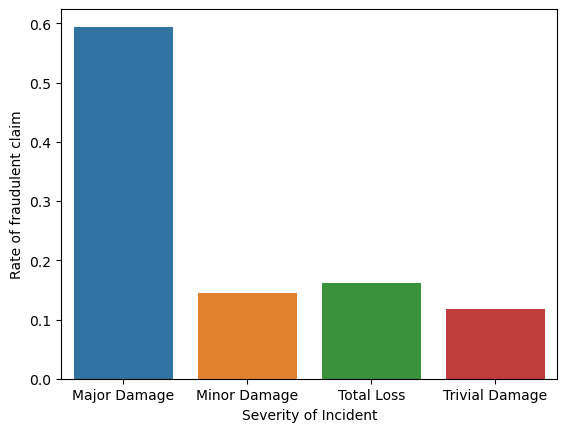
\includegraphics[scale = 0.5]{Severivity.png}
\end{figure}

We can observe that there is a significantly higher rate of fraud among claims with major damage severity. 

\end{frame}

\begin{frame}{Modeling results and analysis (Contribution of Chess hobby)}

\begin{figure}
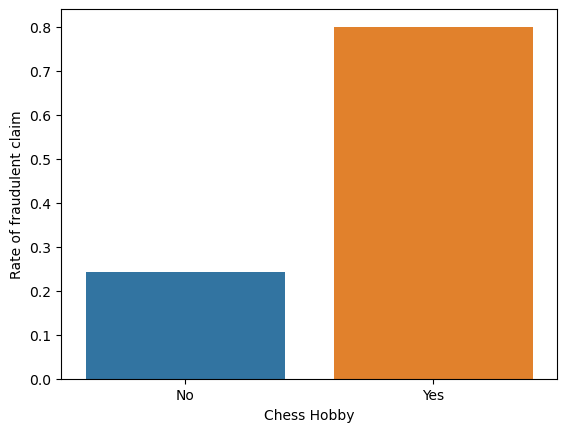
\includegraphics[scale = 0.5]{Chess.png}
\end{figure}

We can observe that there is a significantly higher rate of fraud among claims from people who like playing chess. 

\end{frame}

\begin{frame}{Modeling results and analysis (Contribution of amount of property claims)}

\begin{figure}
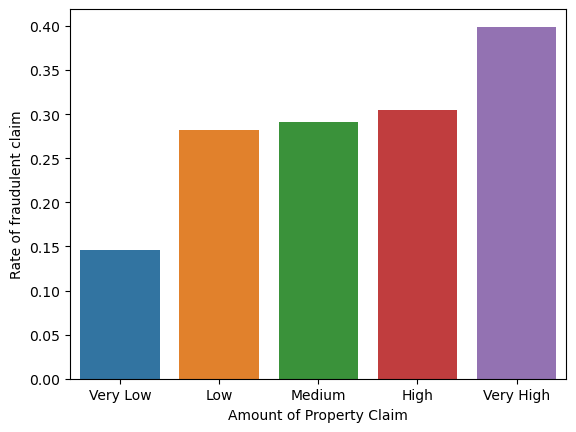
\includegraphics[scale = 0.5]{AOPC.png}
\end{figure}

We can observe that the claims with very low amount of property claims are less likely as fradulent as the ones with very high amount of property claim. 

\end{frame}

\begin{frame}{Modeling results and analysis (Contribution of amount of injury claims)}

\begin{figure}
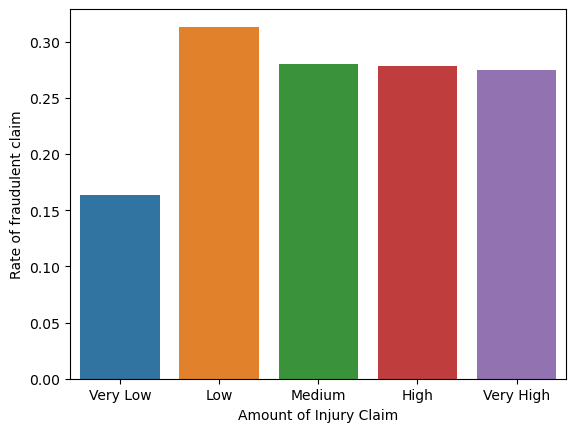
\includegraphics[scale = 0.5]{AOIC.png}
\end{figure}

We can observe that a claims with very low amount of injury claim has a small rate of fraud.

\end{frame}

\begin{frame}{Modeling results and analysis (Contribution of amount of vehicle damage claims)}

\begin{figure}
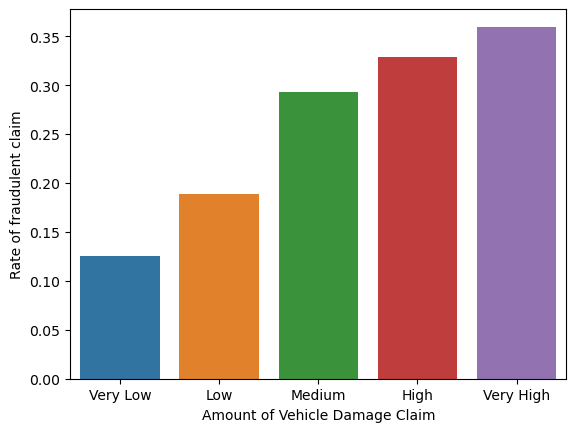
\includegraphics[scale = 0.5]{AOVD.png}
\end{figure}

We can observe that the rate of fraudulent claims is positive correlated to the amount of vehicle damage claim. 

\end{frame}






\begin{frame}
    \Huge{\centerline{The End}}
\end{frame}

%----------------------------------------------------------------------------------------

\end{document}